
\textbf{Disclaimer:} The PyHEADTAIL and Sixtracklib simulation results that are presented in this chapter were performed at a preliminary stage of this project. In  particular they were performed before the thourough analysis of the experimental data which was described in Chapter~\ref{Ch:2018_analyisis}. To this end, the simulations were performed for beam and machine conditions similar to the ones in SPS during the tests with $\CC$s in 2018 but with some small deviations in the bunch length and the beta function on the location of the CC, the value of linear chromaticity and the synchrotron tune. However, it should be highlighted, that since the objective of these studies was to benchmark the theoretical model of T.~Mastoridis and P.~Baudrenghien against different simulation codes these small numerical deviations do not affect the quality of the study. Nevertheless, the simulation studies that will be presented in Chapters~\ref{Ch:investigating_discrepancy} and~\ref{Ch:experimental_CC_2022} were undertaken with more rigorous parameters for the 2018 experiment.
From these plots, it becomes evident that there is an excellent agreement between the theoretically predicted vertical emittance growth and the simulation results with Sixtracklib. Ths results from Sixtracklib simulations are also in agreement with the results from PyHEADTAIL. To this end, it is concluded that taking into account the detailed optics of the SPS cannot explain the discrepancy between expected and measured emittance growth that was observed in the SPS CC tests in 2018.

\section{Parametric studies based on the theoretical model}\label{sec:paramteric_studies_theory}
% Link to presentations: https://docs.google.com/presentation/d/1wqgJK7uDFDGoX8gyx2-JhnO8mZT51N1VH1RtNL-jhWA/edit#slide=id.ga69ead34aa_0_419

The basics of the existing theoretical model which describes the emittance growth in the presence of amplitude and phase noise in the $\CC$s in a synchrotron have been introduced in Chapter~\ref{Ch:CC_noise_theory}. Here, this theory is used to study the sensitivity of the noise-induced emittance growth on the $\CC$ voltage and rms bunch length. The objective of the study is to investigate if the uncertainty in the measurements of these two variables could explain the observed discrepancy of a factor $\sim$4 between measured emittance growth and the analytically predicted values (see Section~\ref{sec:meas_2018_vs_theory}).
% The study is limited in these two parameters as they are the only measured ones that could introduce some incertainty in the Eqs. of phase and amplitude noise. In reality there is also some uncertaninty on the noise levels themselves but is not treated here. Nevertheless, extended studies on the noise spectrum are presented later in this section.

The following parametric studies were performed for the experimental configuration of 2018: beam energy of 270\,GeV, vertical beta function of 73\,m (at the location of $\CC$2), and phase and amplitude noise of -111.4 and -115.7\,dBc/Hz respectively (Coast2-Setting2). The phase and amplitude noise are considered here independently, instead of the effective phase noise, due to the different dependence of the correction term (see Fig.~\ref{fig:correction_term_bunch_length}).

\subsection{Sensitivity to bunch length}\label{subsec:bunch_length_dependence}
Using Eqs.~\eqref{eq:dey_an} and~\eqref{eq:dey_pn} with the above mentioned parameters and CC votlage, $V_\mathrm{CC}$=1\,MV the normalised vertical emittance growth is computed as a function of different values of bunch lengths over a range from $10^{-3}$ to 2.5\,ns (expressed in $4\sigma_t$). The results are illustrated in Fig.~\ref{fig:sensitivity_bunch_length_theory_bunch1}. 

A clear dependence of the vertical emittance growth on the bunch length is observed. However, the dependence is strong for short bunches. In the regime of the measured bunch length during the CC experiment for bunch 1 (~1.6ns-2.0ns) the sensitivity to the bunch length is very small and cannot explain the factor of about 4 that was observed between measurements and simualtions in SPS $\CC$ tests in 2018.

% Plotting script: Requires python 3
% https://github.com/natriant/theoreticalModel_for_emitGrowth_due2CCNoise/blob/master/cmpt_GrowthDependence_on_BunchLength_003_for_thesis.py
\begin{figure}[!h]
    \centering         
    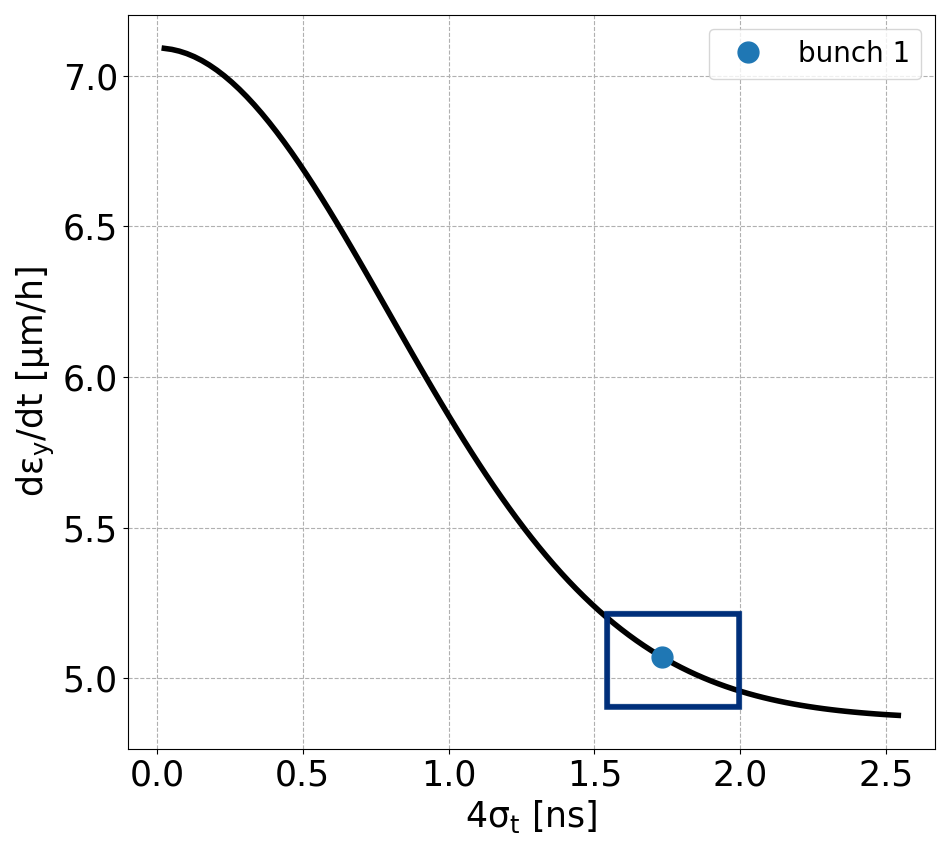
\includegraphics[width=0.7\textwidth]{images/Ch6/dey_vs_4sigmat_Coast2-Setting2_withBunches_v2.png}
        \caption{Vertical emittance growth for different bunch length values computed using the analytical formulas Eqs.~\eqref{eq:dey_an} and~\eqref{eq:dey_pn} for the experimental configuration of 2018. The blue dot shows the average rms bunch length over all coasts in 2018. The blue box around it gives the upper and lower limits of its measurements.}
        \label{fig:sensitivity_bunch_length_theory_bunch1}
 \end{figure}


\subsection{Sensitivity to CC voltage}\label{subsec:bunch_length_dependence}
Here, the sensitivity of the vertical emittance growth is studied for the parameters mentioned above and rms bunch length of $4\sigma_t=$1.7\,ns. The vertical emittance growth is computed again analytically using Eqs.~\eqref{eq:dey_an} and~\eqref{eq:dey_pn} over a range of $\CC$ voltage values equally spaced from 0.6 to 1.3\,MV. 

Figure~\ref{fig:sensitivity_VCC_theory_bunch1} illustrates the computed vertical emittance as a function of the CC voltage. From the analysis in 2018, the calibration of the CC voltage which showed 1\,MV was tricky. However, from the plot it is evident that even if the actual voltage was 30$\%$ lower due to errors this would lead to just a factor of 2 lower vertical emittance growth. An error of this scale is not realistic. To this end, it is concluded that uncertainties on the beam based measurements of the CC voltage cannot explain the expereimental observations of 2018, where there was a factor 4 betewen measured and predicted emittance growth.

% Plotting script: Requires python 3
% https://github.com/natriant/theoreticalModel_for_emitGrowth_due2CCNoise/blob/master/cmpt_GrowthDependence_on_Vcc.py
\begin{figure}[!h]
    \centering         
    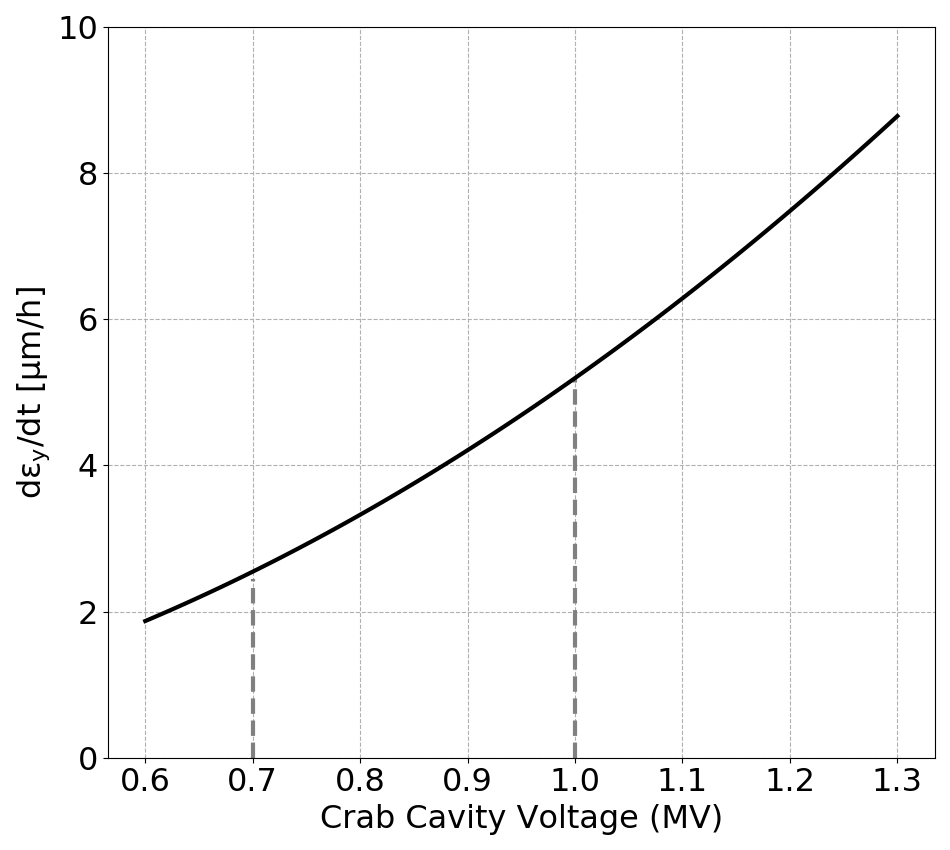
\includegraphics[width=0.7\textwidth]{images/Ch6/dey_vs_Vcc_Coast2-Setting2.png}
        \caption{Vertical emittance growth for different values of CC voltage computed using the analytical formulas Eq.~\eqref{eq:dey_an} and~\eqref{eq:dey_pn} for the experimental configuration of 2018.}
        \label{fig:sensitivity_VCC_theory_bunch1}
 \end{figure}

\section{Benchmarking theory against PyHEADTAIL}\label{sec:benchmark_theory_with_pyheadtail}

% Note on HEADTAIL to PyHEADTAIL: https://www2.kek.jp/accl/legacy/seminar/file/PyHEADTAIL_PyECLOUD_2.pdf
As mentioned in Chapter~\ref{Ch:CC_noise_theory} the available analytical model which predicts the emittance growth driven by CC RF phase and amplitude noise was benchmarked against simulation results with the HEADTAIL~\cite{PhysRevSTAB.18.101001} simulation tool. In this section, the predictions of the model are benchmarked against the PyHEADTAIL simulation tool. PyHEADTAIL is the implementation of the HEADTAIL (which was written in C/C++ language) in Python language in a way that is easier to be maintained and extended~\cite{pyheadtail_schenk}. Further details on the PyHEADTAIL were introduced in the introductory Subseection~\ref{subsec:pyheadtail}.

The parameters used for setting up the linear transfer map, the longitudinal tracking, and the initialisation of the beam distribution are shown in Table~\ref{tab:pyheadtail_simulation_parameters_first_tests} and they are similar to the SPS CC experiments of 2018. The accelerator ring is consisted of one segment, with one interaction point, where the beam receives the noise kicks from the $\CC$ every turn. In particular, at that location, the angle variable, $y^\prime$, of each particle within the bunch is updated every turn following the description of Eqs.~\eqref{eq:amplitude_noise_kick} and~\eqref{eq:phase_noise_kick} for modeling the phase and amplitude noise respectively. The vertical angle co-ordinate is updated to study the vertical emittance growth following the experiments of 2018 where the $\CC$ module that was used provided a vertical deflection to the bunches. Nevertheless, the beam dynamics are the same in the horizontal plane.

The simulations were performed for both phase and amplitude $\CC$ RF noise. The noise level was chosen to be much stronger than the levels used in the experiment of 2018 in order to observe a reasonable growth in the simulation time which was $10^5$ turns. For reference, this corresponds to about 2.5\,s in the SPS machine. Therefore, the simulations were performed for phase and amplitude noise with a power spectral density of 1.68 $\times 10^{-10} \ \mathrm{rad^2/Hz}$ or 1/Hz (for phase and amplitude noise respectively). This corresponds to a scaling factor, $A=10^{-8}$, in Eqs.~\eqref{eq:amplitude_noise_kick} and~\eqref{eq:phase_noise_kick}. 

The power spectra of the sequence of amplitude and phase noise kicks (discrete-time signal) are visualised in Fig.~\ref{fig:psd_cc_simulations_example}. The power spectral densities are computed using Eq.~\eqref{eq:Sxx_definition_discrete_normalized}.

% Plotting scripts: /eos/user/n/natriant/Project_thesis/chapter6/plot_psd_for_simulations_noise.ipynb
\begin{figure}[htp]
    \centering
    \begin{subfigure}{.45\textwidth}
        \centering
        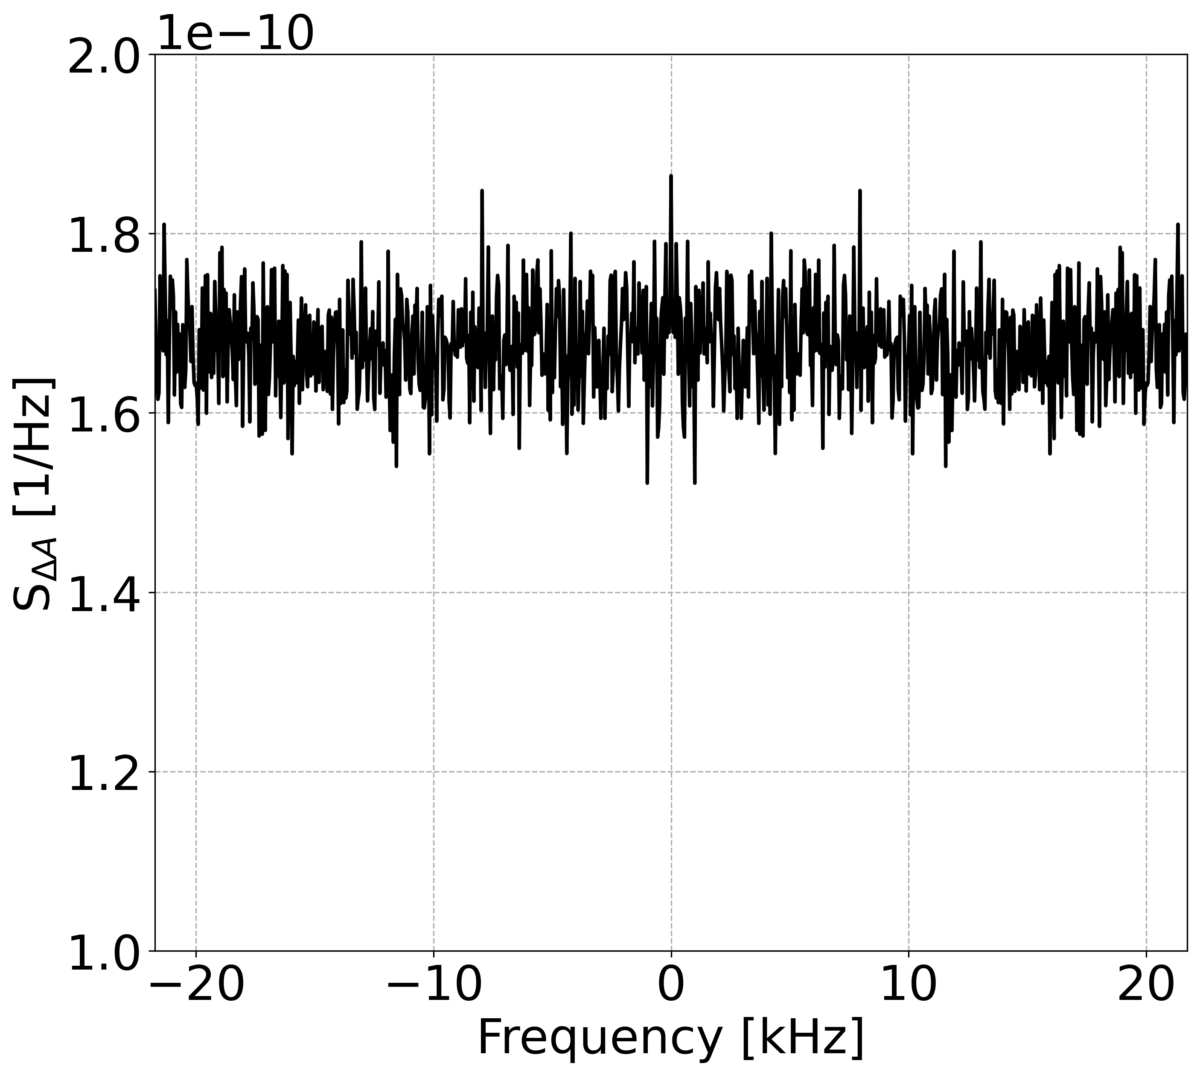
\includegraphics[width=.95\linewidth]{images/Ch6/psd_amplitude_noise_example.png}  
    \end{subfigure}
    \begin{subfigure}{.45\textwidth}
        \centering
        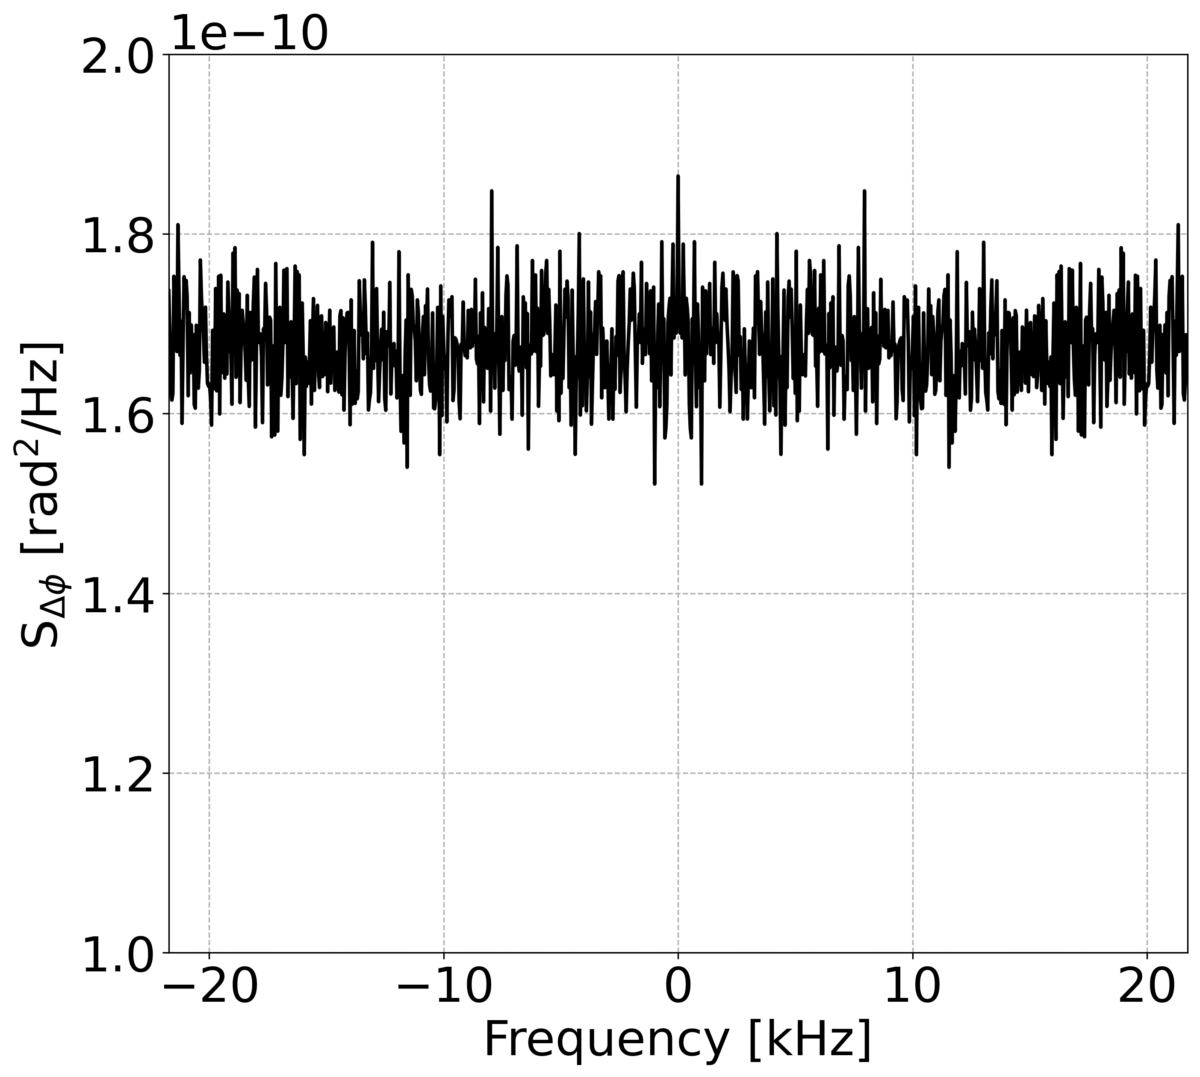
\includegraphics[width=.95\linewidth]{images/Ch6/psd_phase_noise_example.png}
    \end{subfigure}
    \caption{Power sepctrum of the CC amplitude (left) and phase (right) noise used in the PyHEADTAIL simulations.}
    \label{fig:psd_cc_simulations_example}
\end{figure}

The simualtions were performed for a single bunch. The initial bunch was generated with Gaussian distributions in transvserse and longitudinal planes. \footnote{The longitudinal distribution in reality is not a Gaussian but it was found that the longitudinal profile has no significant impact on the predicted emittance growth rates. These studies were performed by T.~Mastoridis and P.~Baudrenghien. \textcolor{red}{There is no reference to these studies. Just Personal communication with a pdf file with the simulation results. How should I state it?} The simualtion studies presented in this thesis used a Gaussian longitudinal distribution following the studies presented in Ref.~\cite{PhysRevSTAB.18.101001}.} 
% Email communication on: 25Nov2020. 
% The attached files in the email can be found in /Documents/Phd_thesis_draft/Ch6 (locally on my mac).
The bunch intensity of $3\times 10^{10}$ protons was represented by $10^5$ macroparticles. 

The beta function at the location of the interaction point was chosen to be the ones at the location of $\CC$1 for both horizontal and vertical planes (values are listed in Table~\ref{tab:pyheadtail_simulation_parameters_first_tests}). The other two Twiss parameters (alpha and dispersion function) were chosen to be zero. This is a valid assumption for the studies since these parameters have no direct impact on the noise-induced emittance growth~\cite{PhysRevSTAB.18.101001}. % It can also be seen in the equations that give the growth.
This is also confirmed, with simulations with the Sixtracklib code which are presented in the following section. The Sixtracklib simulations use the detailed optics of the machine for the tracking. It will be shown that the emittance growth from the two simulated tools are in good agreement.

% Presentation with the comment on the vertical tune distribution: https://docs.google.com/presentation/d/1rBVKGd9aBZTslaAHf48FdJkNPRyXtMF_T9XpEBlLE4c/edit#slide=id.g8ae11a254a_0_952
The mechanism responsible for the emittance growth in the prsesence of noise is the spread of the betatron tunes~\cite{Lebedev:248620}. It is reminded that the tune spread leads to a phase mixing of the particles within the bunch causing a decoherence of the the betatron oscillations which then results to emittance growth~\cite{Lebedev:248620}. The time scale of the decoherence equals the inverse of the betatron frequencies~\cite{Lebedev:248620}: % p.151
\begin{equation}\label{eq:decoherence_time}
    \tau_\mathrm{decoh} = \frac{1}{2\pi \frev \mathrm{rms}(\Delta Q_u)},
\end{equation}
where $u=(x,y)$ indicates the horizontal or vertical plane, $\frev$ the revolution frequency, and $\mathrm{rms}(\Delta Q_u)$ the transverse rms betatron tune spread. The latter can be computed by Eqs.~\eqref{eq:rms_amplitute_detuning_3} and~\eqref{eq:rms_amplitute_detuning_3_x} for the vertical and horizontal planes respectively.

Therefore, it becomes clear that in order to observe some emittance growth a source of tune spread must be included in the simualtions. For the simualtions presented here detuning with transverse amplitude is introduced as described in Section~\ref{subsec:pyheadtail}. It is modeled as a change of the phase advance of each individual particle depending on its action variable and the detuning coefficents. Detuning in the both transverse planes is thus introduced for vertical detuning coefficent $\alpha_\mathrm{xx}=179.35$\,1/m, vertical detuning coefficent $\alpha_\mathrm{yy}=-30.78$\,1/m and for cross-term coefficent $\alpha_\mathrm{yx}=-441.34$\,1/m. These coefficents were computed using MAD-X~\cite{madx} for the nominal SPS lattice (introduced in Section~\ref{sec:optics_model_designs}) and for $Q^\prime{x,y=0.5}$. It should be noted that the detuning in the vertical plane is the value of intereset since the emittance evolution will be investigated in the vertical plane too. Using Eq.~\eqref{eq:rms_amplitute_detuning_3} for the above mentioned coefficents and the initial transverse actions of the bunch, it is computed that $\mathrm{rms}(\Delta Q_y)\approx 7 \times 10^{-6}$. 

For the emittance growth studies to be valid the simulation time should be much longer than decoherence time defined in Eq.~\eqref{eq:decoherence_time}. For the above value of rms vertical tune spread, the decoherence time is computed to be: $\tau_\mathrm{decoh} \approx 0.5$\,s. Therefore, the simualtion time of about 2.5\,s is reasonable for these studies.
% from MAD-X for no b3b5b7 and QpcQPy=0--> axx=170.65, ayy = -29.70 and axy = -440.87.


% For the compaction factor I am not sure but it doesn't matter
% The chromaticity value was not 5e-1 for all the simulations. For some of the cases was 5e-1, for some others was 2 etc. However, it doesn't matter.
\begin{table}[!hbt]
	\begin{minipage}{\textwidth}
      \begin{centering}
   \caption{Simulation parameters used to benchmark the theoretically predicted emittane growth in Chapter~\ref{Ch:investigating_discrepancy}.}
	\begin{tabu} to \textwidth {X[c,m] X[0.5c,m] X[0.5c,m] X[0.01c,m]}
		&&& \\[-6mm]
		\toprule \toprule
		\multicolumn{2}{l}{\textbf{Parameter}} &
		\multicolumn{2}{c}{\textbf{Value}} \\
		\bottomrule
      \multicolumn{2}{l}{Beam energy, $\symE$} & \multicolumn{2}{c}{270\,GeV} \\
      \multicolumn{2}{l}{Machine circumference, $C_0$}  & \multicolumn{2}{c}{6911.5623\,m} \\
      \multicolumn{2}{l}{Horizontal / Vertical betatron tune, $\Qx$ / $\Qy$}  & \multicolumn{2}{c}{26.13 / 26.18} \\
      %\multicolumn{2}{l}{Horizontal / Vertical linear chromaticity, $Q^\prime_x$ / $Q^\prime_y$}  & \multicolumn{2}{c}{0.5 / 0.5} \\
      \multicolumn{2}{l}{Synchrotron tune, $\Qs$}  & \multicolumn{2}{c}{0.0035}\\
      \multicolumn{2}{l}{Momentum compaction factor, $\alpha_p$}  & \multicolumn{2}{c}{1.9 $\times 10^{-3}$}\\
      \multicolumn{2}{l}{Number of bunches}  & \multicolumn{2}{c}{1} \\
      \multicolumn{2}{l}{Rms bunch length, $\sigma_z$}  & \multicolumn{2}{c}{15.5\,cm}\\
      \multicolumn{2}{l}{Horizontal / Vertical normalised emittance, $\epsilon_x$ / $\epsilon_y$}  & \multicolumn{2}{c}{2\,$\mathrm{\mu m}$ / 2\,$\mathrm{\mu m}$}\\
      \multicolumn{2}{l}{Horizontal / vertical beta function, $ \beta_{x, CC1} / \beta_{y, CC1}$}  & \multicolumn{2}{c}{29.24\,m / 76.07\,m $^\dagger$ } \\
      \bottomrule
      \multicolumn{2}{l}{Number of macroparticles, $N_\mathrm{mp}$}  & \multicolumn{2}{c}{$10^5$} \\
      \multicolumn{2}{l}{Number of turns, $N_\mathrm{slices}$}  & \multicolumn{2}{c}{$10^5$} \\
      \bottomrule
	\end{tabu}
   \label{tab:pyheadtail_simulation_parameters_first_tests}
   \end{centering}\footnotesize{\\ $^\dagger$ Model values for the Q26 optics.}
   \end{minipage}
\end{table}



% Slides where the plots were taken from: https://docs.google.com/presentation/d/1xK63pVRDlW1KIV2NE3UMlAL3VnjhegwjbkpC0ufSpjg/edit#slide=id.g72167b2e95_0_70
% They can also be found at: https://docs.google.com/presentation/d/1WgxpGTsyy55XtOVT1ea9u3SO9EyG5EQMWuqhLyM46mM/edit#slide=id.g727b0ea384_1_7
\begin{figure}[htp]
    \centering
    \begin{subfigure}{.45\textwidth}
        \centering
        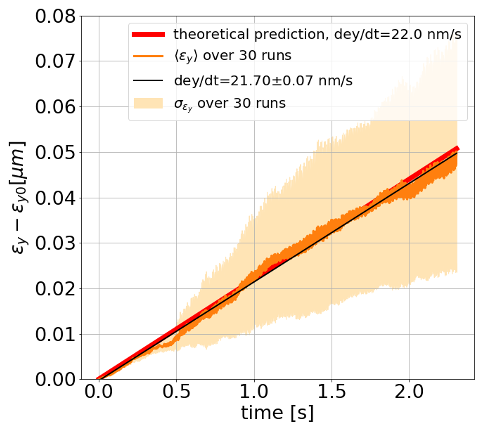
\includegraphics[width=.95\linewidth]{images/Ch6/pyheadtail_benchmark_amplitude_noise.png}  
    \end{subfigure}
    \begin{subfigure}{.45\textwidth}
        \centering
        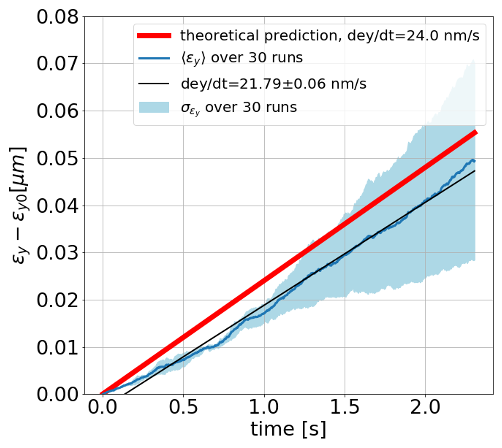
\includegraphics[width=.95\linewidth]{images/Ch6/pyheadtail_benchmark_phase_noise.png}
    \end{subfigure}
    \caption{Vertical emittance growth driven by CC RF amplitude noise (left) and phase noise (right) as simulated with PyHEADTAIL simulation tool for a configuration close to the experimental conditions of the SPS CC tests in 2018.}
    \label{fig:study_pyheadtail_normalised_momentum_kicks}
\end{figure}




\section{Benchmarking theory against Sixtracklib}\label{sec:benchmark_theory_with_sixtracklib}
This section summarises the benchmarks that were made to validate the theoretical model~\cite{PhysRevSTAB.18.101001} against numerical simulations with Sixtracklib~\cite{sixtracklib_repo} which is a non-linear single-particle tracking library. The idea is motivated by the fact that PyHEADTAIL and theory may miss some beam dynamics that could explain the discrepancy between their results and the experimental observations of 2018. Sixtracklib is a more complete simulation tool than PyHEADTAIL as the tracking simulations use the detailed optics of the machine and therefore is considered appropriate for this study. Calculations can be performed on GPU decreasing the computational time. For all the simulations presented in this section the nominal SPS model for Q26 optics will be used~\cite{cern_optics_repo} as introduced in Section~\ref{sec:optics_model_designs} except if it is stated otherwise.


This section is structured as follows. First, a direct comparison between PyHEADTAIL and Sixtracklib is provided by simulating the emittance growth for the experimental conditions of 2018. In the Sixtracklib simulations, the available $\CC$ element is used instead of modeling only the transverse kicks on the angle co-ordinate due to phase and amplitude noise in the RF system of the cavity as in PyHEADTAIL. Afterward, the sensitivity of the noise-induced emittance growth in the multipole errors of the main SPS dipoles is tested. Furthermore, the simulations are performed using the measured noise spectra of amplitude and phase noise. Last, the sensitivity of the emittance growth to a possible $\CC$ phase modulation is studied.

\subsection{Implementation of CC element in Sixtracklib}\label{subsec:sixtracklig_CC_implementation}
% Link to corresponding presentation:https://docs.google.com/presentation/d/15038dO7vsEUYxzCsYtQXYlpRIwtVGkA8esGtvKHwBwM/edit#slide=id.g6da2141836_0_5
Sixtracklib provides the possibility to perform tracking simulations in the presence of an actual $\CC$ element on which noise can be added, instead of modeling only the transverse momentum kicks due to phase and amplitude noise in the RF system of the cavity like in PyHEADTAIL.

In Sixtracklib the $\CC$ element is represented by an element (referred to as RFMultipole in the Sixtracklib documentation) that has the properties of an RF cavity and of a magnet of arbitrary order oscillating at a certain frequency. To simulate the vertical $\CC$ it is implemented as a (modulated) skew dipole.

When a particle passes through this element, it recieves the following vertical kick on the momentum:
\begin{equation}\label{eq:CC_kick_sixtracklib_vertical}
    y^\prime_{j+1} = y^\prime_{j} + \cos{\left ( \phi_\mathrm{CC} \frac{\pi}{180} - \frac{2\pi f_\mathrm{CC}}{c} \frac{z \beta_0}{\beta^2} \right )} \frac{V_\mathrm{0,CC}}{p_0 c},
\end{equation}
where $j={0, ...., N_\mathrm{turns}}$ denotes the turn number with $N_\mathrm{turns}$ being the total number of turns that the beam passes through the element. Furthermore, $y^\prime$ is the vertical angle co-ordinate and z the longitudinal co-ordinate of each particle, $\phi_\mathrm{CC}$ the $\CC$ phase in degrees, $f_\mathrm{CC}$ is the $\CC$ frequency, $c$ is the speed of light, $\beta_0$ is the relativistic beta, $V_\mathrm{0,CC}$ is the amplitude of the $\CC$ voltage and $p_0$ the reference momentum.


Before using this element for the emittance growth simulations its implementation in Sixtracklib was tested. This check was important as Sixtracklib is a recently developed simulation tool and at the time these studies took place the use of the RFMultipole as a $\CC$ element was not well tested. The $\CC$ element installed at a location $s_0$, acts like a single dipole field error at a different location, $s_1$, around the ring. To this end, the induced orbit shift at the location $s_1$ from the $\CC$ element is benchmarked against the theoretically expected orbit shift resulting from a single dipole field error. The latter has already been discussed in the context of the reconstruction of $\CC$ voltage from the HT monitor in Section~\ref{sec:Vcc_calibration}. Equation~\eqref{eq:CC_orbit_shift_CC_element}, which is obtained from Eq.\,(1) from chapter 4.7.1 in Ref.~\cite{Chao:1490001}, gives the vertical orbit shift (in meters) from the $\CC$ kick (at the location $s_0$), at the location $s_1$ as follows:

\begin{equation}\label{eq:CC_orbit_shift_CC_element}
    \Delta y_{,s_11} = \frac{\sqrt{\beta_{y, s_1}}}{2 \sin(\pi \Qy)} \Delta y^\prime \sqrt{\beta_{y, s_0}} \cos(\pi \Qy - \mid \psi_{y, s_1} - \psi_{y, s_0} \mid),
 \end{equation}
where $\Delta y^\prime=y^\prime_{j+1}-y^\prime_{j}$, where $j$ is the number of turns for which the tracking is performed, $\Qy$ is the vertical tune, $\beta_{y, s_0}$ and $\beta_{y, s_1}$ the vertical beta function at the locations $s_0$ and $s_1$ respectively and $\mid \psi_{y, s_1} - \psi_{y, s_0} \mid)$ is the vertical phase advance in tune units between the locations $s_0$ and $s_1$.

Figure~\ref{fig:sixtracklib_CC_orbit_shift_vs_theory} compares the shift of the orbit as computed analytically using Eq.~\eqref{eq:CC_orbit_shift_CC_element} (blue) for the values reported in Table~\ref{tab:SPS_CC_WS_sixtracklib} and as obtained from Sixtracklib simulations (orange). The induced orbit shift was obtained from Sixtracklib simulations after tracking 1000 particles for 500 turns in the presence of the above-mentioned CC element (which is installed at the location of $\CC$1). The simulations took place using an initial Gaussian bunch distribution in the six-dimensional phase space. The initial normalised emittances were $\epsilon_x$=2.5\, $\mathrm{\mu m}$ and $\epsilon_x=2.5 \times 10^{-6}$\, $\mathrm{\mu m}$ for the horizontal and vertical plane respectively. The distribution was chosen to be so small in the vertical plane so there is practically no initial offset which facilitates the observation of the orbit shift. % If we had offset we would need to split in longitudinal slices and take the average position of each slice.
 The location $s_1$ was set at the start of the lattice which for this study it was considered to be the horizontal rotational Wire Scanner, BWS.51995.H. This choice was arbitrary. The most relevant simulation parameters are listed in Table~\ref{tab:SPS_CC_WS_sixtracklib}.
% Note: The induced closed orbit shown in the plot corresponds to the start of the lattice (BWSA.51995) as the particles are dumped in that location. Link to complementary slides: https://docs.google.com/presentation/d/1-w9CRX_IuH6tWqg7Mx450sDhk7hBIXyBsZ0hyumq4hw/edit#slide=id.g6d31fa0069_1_14


% Image downloaded from: https://docs.google.com/presentation/d/15038dO7vsEUYxzCsYtQXYlpRIwtVGkA8esGtvKHwBwM/edit#slide=id.g6da5555eb3_1_59
\begin{figure}[!h]
    \centering         
    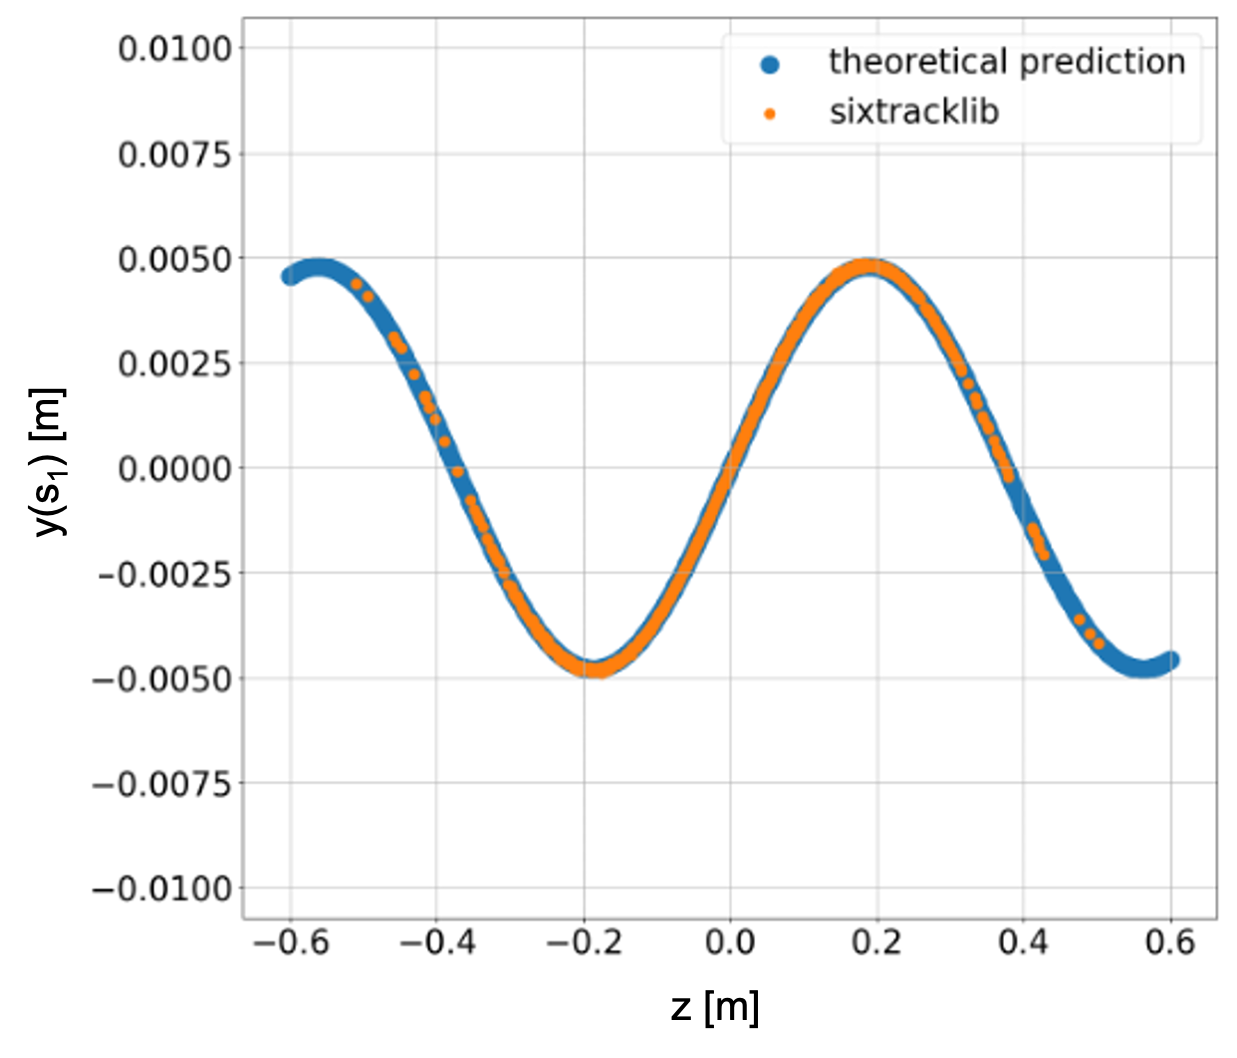
\includegraphics[width=0.7\textwidth]{images/Ch6/Vcc_orbit_shfit_sixtracklib_sanity_check.png}
        \caption{Vertical orbit shift at the location of the horizontal Wire Scanner (SPS.BWS.51995.H.) induced by the CC element as computed analytically (blue) and from tracking simulations with Sixtracklib (orange).}
        \label{fig:sixtracklib_CC_orbit_shift_vs_theory}
\end{figure}

% Optics were taken from: https://github.com/natriant/rf_multipole_sanity_checks/blob/master/pysixtrack/rf_multipole_sanity_check_pysixtrack_001.ipynb
\begin{table}[!hbt]
	\begin{minipage}{\textwidth}
   \begin{centering}
   \caption{Parameters for computing the vertical orbit shift induced by the CC element (at the location $s_0$) at the location of the horizontal Wire Scanner (SPS.BWS.51995.H.), $s_1$.}
	\begin{tabu} to \textwidth {X[c,m] X[0.01c,m] X[0.01c,m] X[0.01c,m]}
		&&& \\[-6mm]
		\toprule \toprule
		\multicolumn{2}{l}{\textbf{Parameter}} &
		\multicolumn{2}{c}{\textbf{Value}} \\
		\bottomrule
      \multicolumn{2}{l}{Beta function at the Wire Scanner, $\beta_{y, s_1}$}& \multicolumn{2}{c}{27.47\,m} \\
      \multicolumn{2}{l}{Phase advance to the Wire Scanner$^{\ast}$, $\psi_{y, HT}$} & \multicolumn{2}{c}{0} \\
      \multicolumn{2}{l}{Beta function at the $\CC$1, $\beta_{y, CC1}$}& \multicolumn{2}{c}{76.07\,m} \\
      \multicolumn{2}{l}{Phase advance to the $\CC$1$^{\ast}$, $\psi_{y, CC1}$} & \multicolumn{2}{c}{4.05 $\times$ 2$\mathrm{\pi}$} \\
      \multicolumn{2}{l}{Vertical betatron tune, $\Qy$} & \multicolumn{2}{c}{26.18} \\
      \multicolumn{2}{l}{Beam energy, $\symE$} & \multicolumn{2}{c}{26\,GeV} \\
      \multicolumn{2}{l}{rms bunch length, $\sigma_z$} & \multicolumn{2}{c}{0.22\,m} \\
      \multicolumn{2}{l}{rms momentum spread, $\sigma_\delta$} & \multicolumn{2}{c}{1e-4} \\
      \multicolumn{2}{l}{CC voltage, $V_\mathrm{0,CC}$} & \multicolumn{2}{c}{3\,MV} \\
      \multicolumn{2}{l}{CC frequency, $f_\mathrm{CC}$} & \multicolumn{2}{c}{400\,MHz} \\
      \multicolumn{2}{l}{CC phase, $\phi_\mathrm{CC}$} & \multicolumn{2}{c}{90\,deg$^{\dagger}$} \\
      \bottomrule
	\end{tabu}
   \label{tab:SPS_CC_WS_sixtracklib}
   \end{centering} \footnotesize{$^\ast$ The phase advances are measured from the start of the lattice which is considered the element SPS.BWS.51995.H that is the horizontal rotational Wire Scanner. \\$^\dagger$ It was found that in the definition of the RFMultipole the phase of the cavity is shifted by 90 degrees compared to the standard (theoretical) crab cavity kick.}
   \end{minipage}
\end{table}

For the computation of the theoretical prediction Eq.~\eqref{eq:CC_orbit_shift_CC_element} was used over a range of equally spaced $z$ co-ordinates from -0.6 to 0.6\,m ($\sim 3 \sigma_z$). The $z$ co-ordinates are taken into account indirectly through $\Delta_y^\prime$ and Eq.~\eqref{eq:CC_kick_sixtracklib_vertical}.

By looking at Fig.~\ref{fig:sixtracklib_CC_orbit_shift_vs_theory} it is concluded, that using Sixtracklib the result of $\CC$ element on the orbit is as expected. % on the closed orbit


\subsection{Emittance growth simulations with CC noise modeled as transverse kicks on the angle co-ordinate.}\label{subsec:sixtracklib_kicks_transverse_angle}
% Link to presentation with relevant slides: https://docs.google.com/presentation/d/1rBVKGd9aBZTslaAHf48FdJkNPRyXtMF_T9XpEBlLE4c/edit#slide=id.g8a041cb470_0_448
For the first benchmark, the $\CC$ element was not implemented yet. Instead, the emittance growth was simulated for the simpler case for which the $\CC$ noise which was implemented as an update of the angle, $y^\prime$ of each particle within the bunch, according to the kicks of Eqs.~\eqref{eq:amplitude_noise_kick} and~\eqref{eq:phase_noise_kick} for amplitude and phase noise respectively. The $\CC$ RF noise kicks were applied on the beam at the location of $\CC$1 for which the vertical beta function is 76.07\,m. The scaling factor, $A$, equals $10^{-8}$ which corresponds to $1.68 \times 10^{-10} \ \mathrm{rad^2/Hz}$ or 1/Hz for phase and amplitude noise respectively.

For the simulation setup, beam and machine conditions similar to the $\CC$ experiment of 2018 were used and are listed in Table~\ref{tab:sixtracklib_simulation_parameters}.

\begin{table}[!hbt]
	\begin{minipage}{\textwidth}
      \begin{centering}
   \caption{Sixtracklib simulation parameters used to benchmark the theoretical model of T.~Mastoridis and P.~Baudrenghien~\cite{PhysRevSTAB.18.101001}.}
	\begin{tabu} to \textwidth {X[c,m] X[0.5c,m] X[0.5c,m] X[0.01c,m]}
		&&& \\[-6mm]
		\toprule \toprule
		\multicolumn{2}{l}{\textbf{Parameter}} &
		\multicolumn{2}{c}{\textbf{Value}} \\
		\bottomrule
      \multicolumn{2}{l}{Beam energy, $\symE$} & \multicolumn{2}{c}{270\,GeV} \\
      \multicolumn{2}{l}{Horizontal / Vertical betatron tune, $\Qx$ / $\Qy$}  & \multicolumn{2}{c}{26.13 / 26.18} \\
      \multicolumn{2}{l}{Horizontal / Vertical linear chromaticity, $Q^\prime_x$ / $Q^\prime_y$}  & \multicolumn{2}{c}{0 / 0} \\
      \multicolumn{2}{l}{Synchrotron tune, $\Qs$}  & \multicolumn{2}{c}{0.0035}\\
      \multicolumn{2}{l}{Number of bunches}  & \multicolumn{2}{c}{1} \\
      \multicolumn{2}{l}{Rms bunch length, $\sigma_z$}  & \multicolumn{2}{c}{15.5\,cm }\\
      \multicolumn{2}{l}{Horizontal / Vertical normalised emittance, $\epsilon_x$ / $\epsilon_y$ $^\ast$}  & \multicolumn{2}{c}{2\,$\mathrm{\mu m}$ / 2\,$\mathrm{\mu m}$}\\
      \bottomrule
      \multicolumn{2}{l}{Number of macroparticles, $N_\mathrm{mp}$}  & \multicolumn{2}{c}{$1 \times 10^5$} \\
      \multicolumn{2}{l}{Number of turns, $N_\mathrm{turns}$}  & \multicolumn{2}{c}{$1 \times 10^5$} \\
      \bottomrule
	\end{tabu}
   \label{tab:sixtracklib_simulation_parameters}
   \end{centering}\footnotesize{$^\ast$ Initial values at the start of the tracking.}
   \end{minipage}
\end{table}

The nominal SPS lattice of MAD-X is used: dipoles, quadrupoles, and chromatic sextupoles as discussed in Section~\ref{sec:optics_model_designs}. It can be found in the GitLab repository of Ref.~\cite{cern_optics_repo}. The initial distribution of $10^5$ particles follows a gaussian both in transverse and longitudinal planes. In reality, the distribution in the longitudinal plane is not gaussian. However, it is a very good approximation for this kind of study. \textcolor{red}{Why?}


For the above mentioned machine conditions the expected growth rate is expected to be $\sim$ 22\,nm/s and $\sim$ 24\,nm/s in the presence of phase and amplitude noise respectively. These rates were computed using Eqs.~\eqref{eq:dey_an} and~\ref{eq:dey_pn} respectively.

% Actual emittance definition used in sixtracklib simulations: https://docs.google.com/presentation/d/1rcSwhZBLZi0Js9jeFiVSLzR6HxhzljYkLLrBMahdqus/edit#slide=id.g6e85dffc41_2_60 . It has been shown that is gives the same results with pyheadtail (don't remember the date of the corresponding slides).

The bunch was tracked for $10^5$ and the normalised emittance was computed every 100 turns (for computational efficiency) using the statistical defintion defined in Eq.~\eqref{eq:geometric_emittance_v2} and then inserting the value in Eq.~\eqref{eq:normalised_emittance}. To reduce the uncertainty of the results, thirty different simulation runs were undertaken. For every run, the initial bunch distribution and the sequence of the uncorrelated noise kicks were regenerated randomly (a different seed was used in the random generator). 

Figure~\ref{fig:study_1_sixtracklib_normalised_momentum_kicks} illustrates the simulated emittance growth driven by phase (left) and amplitude (right) noise. For both types of noise, the theoretical predicted growth is given with the red line. The dark blue and dark orange lines show the evolution of the averaged emittance values over the thirty different runs. The shaded areas, shown with light blue and light orange colors, depict the standard deviation of the emittance values over the thirty different runs. The emittance growth rate is obtained with a linear fit to the averaged normalised emittance values over the simulation time. The resulted slope of the fit is also shown in the plot with black color. The uncertainty on the slope of the fit is displayed in the legend.

\begin{figure}[htp]
    \centering
    \begin{subfigure}{.45\textwidth}
        \centering
        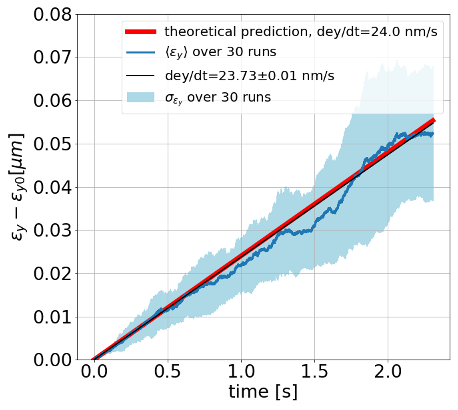
\includegraphics[width=.95\linewidth]{images/Ch6/sixtracklib_study_1_CC_PN_normalised _kicks_in_momentum.png}  
    \end{subfigure}
    \begin{subfigure}{.45\textwidth}
        \centering
        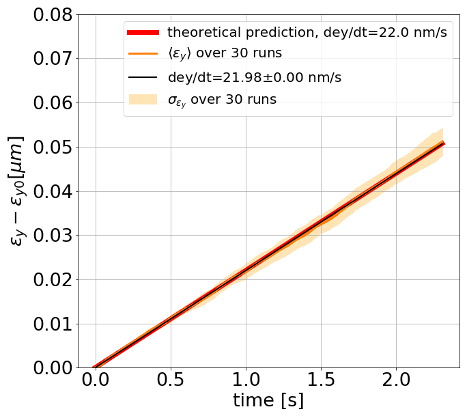
\includegraphics[width=.95\linewidth]{images/Ch6/sixtracklib_study_1_AN_normalised_kicks_momentum.png}
    \end{subfigure}
    \caption{Vertical emittance growth driven by CC RF phase noise (left) and amplitude noise (right) as simulated with Sixtracklib simulation tool for a configuration close to the experimental conditions of the SPS CC tests in 2018. The CC noise is modeled as uncorrelated kicks on the angle variables of the particle every turn following Eqs.~\eqref{eq:phase_noise_kick} and.~\eqref{eq:amplitude_noise_kick} for phase and amplitude noise respectively.}
    \label{fig:study_1_sixtracklib_normalised_momentum_kicks}
\end{figure}

From these plots, it becomes evident that there is an excellent agreement between the theoretical predicted vertical emittance growth and the simulation results with Sixtracklib. Ths results from Sixtracklib simulations are also in agreement with the results from PyHEADTAIL. To this end, it is concluded that taking into account the detailed optics of the SPS cannot explain the discrepancy between expected and measured emittance growth that was observed in the SPS CC tests in 2018.

Another observation, is that the spread between the emittance values obtained from the different runs is much larger in the case of phase noise (left) than in the case of amplitude noise (right). The reason for this is not yet well understood. \textcolor{red}{Further comments are needed here?}

% Presentation with the comment on the vertical tune distribution: https://docs.google.com/presentation/d/1rBVKGd9aBZTslaAHf48FdJkNPRyXtMF_T9XpEBlLE4c/edit#slide=id.g8ae11a254a_0_952
%Last, it is worth commenting on the vertical betatron distribution that was present in the simualtions. As discussed in Chapter~\ref{Ch:CC_noise_theory} the emittance growth driven by $\CC$ RF noise depends on the overlap of the noise spectrum and the betatron tune distribution. For the white noise case (which is the case here) the power spectral density (PSD) is constant within the betatron spread and therefore the effect of noise is independent of the actual tune distribution. Furthermore, for the theoretical model to be valid the simulation time should be much longer than the inverse betatron tune spread~\cite{PhysRevSTAB.18.101001}. This means that for the simulation time (in turns) needs to be much longer than the inverse betatron tune spread,$\mathrm{rms(\Delta Q_y)}$. For nominal SPS lattice (which is used in the simulations) and $Q^\prime{x,y=0.0}$ this is computed to be $\mathrm{rms(\Delta Q_y)} = 7\times 10^{-6}$ \footnote{For the nominal SPS lattice and for $Q^\prime{x,y=0.0}$ the vertical and cross-term detuning coefficents are computed with MAD-X~\cite{madx} as follows: $\alpha_\mathrm{yy}$=-29.7\,1/m and $\alpha_\mathrm{yy}$=-440.87\,1/m.  $mathrm{rms(\Delta Q_y)}$ is computed using Eq.~\eqref{eq:rms_amplitute_detuning_3}. The emittance values are listed in Table~\ref{tab:sixtracklib_simulation_parameters}.}. Therefore. It is not.... from these computations I would need five times longer simulations.
% from MAD-X for no b3b5b7 and QpcQPy=0--> axx=170.65, ayy = -29.70 and axy = -440.87.

%Studies with more realistic tune spread for the experiments of 2018 are presented in Chapter 7.


\subsection{CC noise induced emittance growth in the presence of global CC scheme}\label{subsec:global_CC}






an RFMultipole element which  has the properties of an RF-cavity and of a magnet of arbitrary order oscillating at a certain frequency. To simulate the vertical CC kick we use it as a modulating (skew) dipole.



\subsection{CC noise induced emittance growth in the presence of local CC scheme}\label{subsec:local_CC}

\newpage



ty. The
benchmarks prove an excellent agreement and demonstrate a solid understanding of the involved
dynamics. The study has been published in Ref. [34].


for the experimental configuration of 2018 

of the existing Vlasov theory for transverse coherent beam instabilities with first-order
chromaticity have been recapitulated in Section 2.2.3. Here, we extend this theory to account for the
beam dynamics effects introduced by nonlinear chromaticity. The chapter contains the work published
in Refs. [34, 76].




\section{Benchmarking with different simulation software}
Benchmarking of theory with pyheadtail (one turn map) and Sixtracklib (element by element tracking).



\subsection{PyHEADTAIL}
- real CC element
- local vs global cc scheme
- How emittance is computed. No dipsersive contribution. studies vertical plane. \\
- It was verified in Sixtracklib simulations that the result from this simplified implementation is equivalent to the simulation with the true CC kick including phase noise.\\
- Need to say why in the simulations we have excitation of only the first betatron sideband. \\
\subsection{Sixtracklib}

Remember that in chapter 6 it was demonstrated that there is no visible difference on the cc rf noise induced emittance growth if the noise kicks are modeled as kicks on the moemntum or the real rf multiple + used in a global or local scheme.


pyheadtail vs sixtracklib: %https://docs.google.com/presentation/d/1rBVKGd9aBZTslaAHf48FdJkNPRyXtMF_T9XpEBlLE4c/edit#slide=id.g8ae11a254a_0_701

\section{Sensitivity to the non-linearities of the main SPS dipoles}
Simulation studies with sixtracklib

\section{Simulations using the measured noise spectrum}
Sixtracklib PyHEADTAIL and the exact machine paramters

\section{Sensitvity studies}
1. Sensitvity to how noisy is the noise spectrum
2. On the CC voltage
3. On the different bunch lengths. 

\section{b3b5b7 multiple errors}
Contribution of the non-linearities with sixtracklib.


All these factors were excluded as possible sources of the discrepancy.